
\section[Sobre \LaTeX]{Um pouco sobre \LaTeX}
\setbeamercolor{structure}{fg=slideBlue}
	\begin{frame}{Breve história}
		\begin{itemize}[<+->]
			\item Deriva diretamente do \TeX{}, que foi criado por Donald Knuth, acerca de 1978, queria seus livros saindo das editoras mais bonitos
			\item \TeX{} \textrightarrow{} do grego $\techn$ (téchni), ``artes manuais''
			\item Adaptado por Leslie B. Lamport, com primeiro lançamento em 1983
			\item Consiste em um conjunto de macros que simplificam o uso de \TeX{}
			\item \LaTeX{} \textrightarrow{}  Lamport's $\techn$ \textrightarrow{} $\latec$
			\item Para mais informações: \usebeamercolor[fg]{title}{\href{https://en.wikipedia.org/wiki/LaTeX}{Wikipédia}}
		\end{itemize}
	\end{frame}

    \subsection{\LaTeX{} vs MSWord}
	\begin{frame}{\LaTeX{} vs MSWord}
		\begin{columns}
		    \begin{column}{0.5\linewidth}
		        \emph{\LaTeX{}}:
        		\begin{itemize}[<+->]
                    \item É \textit{Open Source}
                    \item É gratuito
                    \item É lindo
                    \item Fácil de manter controle
                    \item WYSI\textbf{\usebeamercolor[fg]{title}{N}}WYG
                    \item Pra fazer coisas complexas
                    \item \textit{Furute Proof}: compatível com todas as versões futuras
        		    \item Anti-intuitivo para objetos
                \end{itemize}
            \end{column}
            \begin{column}{0.5\linewidth}
                \emph{MSWord}:
                \begin{itemize}[<+(-8)->]
                    \item É \textit{Closed Source}
                    \item É pago
                    \item Não é lindo
                    \item Explode em 10 páginas
                    \item WYSIWYG
                    \item Pra fazer coisas simples
                    \item \textit{Furute Obsolete}: incompatível com versões futuras
        		    \item Intuitivo para objetos
                \end{itemize}
            \end{column}
        \end{columns}
	\end{frame}

	\begin{frame}
    	\begin{figure}[!h]
		    \centering
			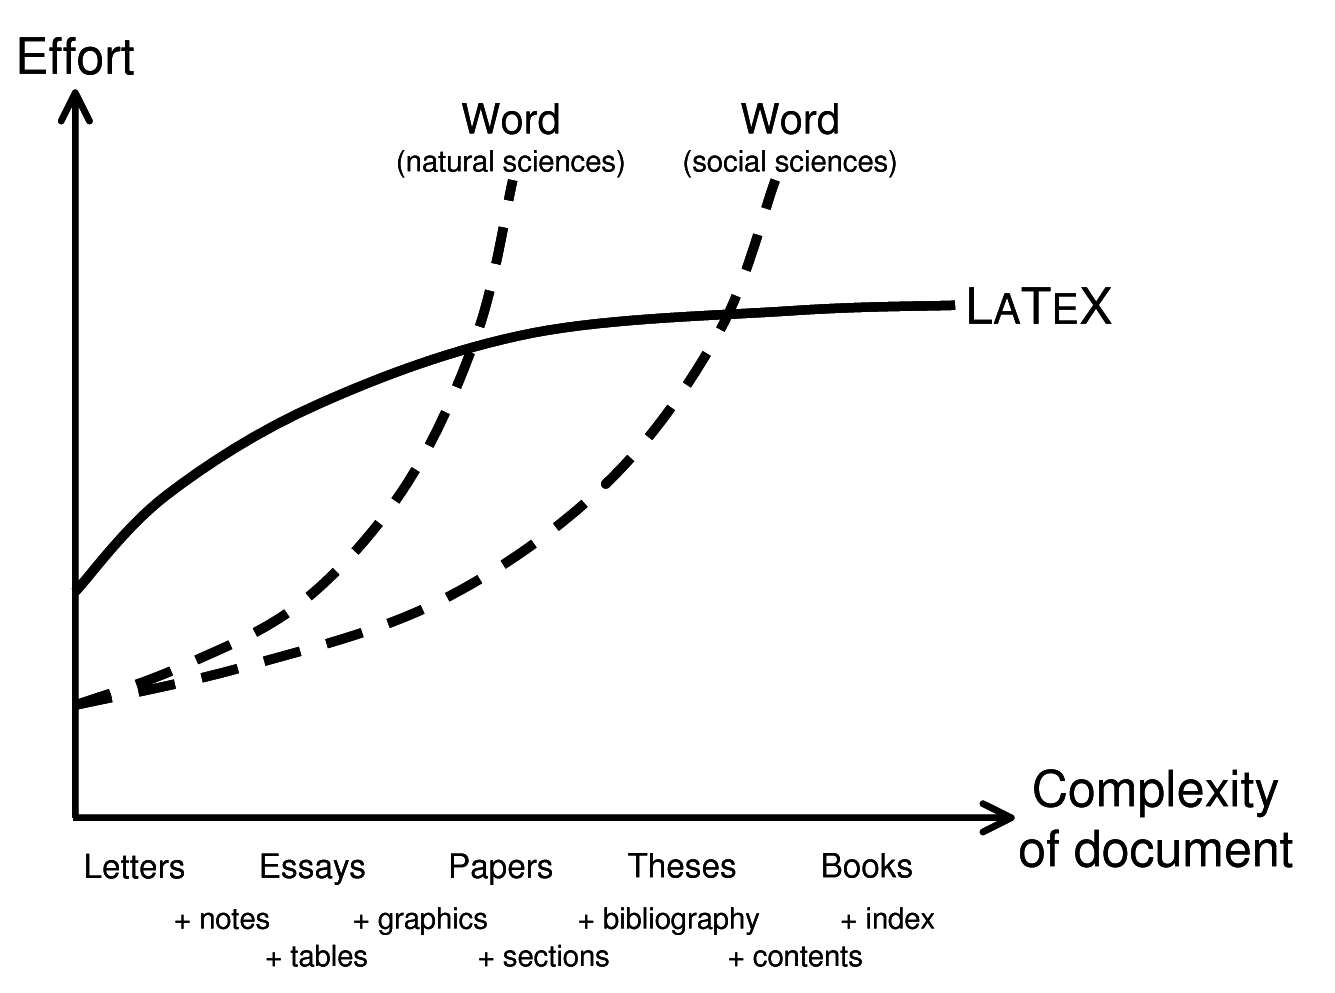
\includegraphics[height=0.95\textheight]{image/LaTeX_vs_MSWord.jpg}
    	\end{figure}
	\end{frame}

	\begin{frame}
    	\begin{center}
    	    WYSIWYG vs WYSI\textbf{\usebeamercolor[fg]{title}{N}}WYG
    	\end{center}
    	\begin{figure}[!h]
		    \centering
			\includesvg[height=0.85\textheight]{image/WYSINWYG}
    	\end{figure}
	\end{frame}

	\subsection{Um código mínimo}
	\begin{frame}{Um código mínimo}
        \begin{columns}
            \begin{column}{0.5\textwidth}
        		\lstinputlisting{../code/basic.tex}
            \end{column}
            \pause
            \begin{column}{0.5\textwidth}
        		\fbox{\begin{minipage}[c][0.8\textheight][t]{0.9\textwidth}
                    \centering
                    \vspace{0.05\textwidth}
                    \begin{columns}
                        \begin{column}{0.8\textwidth}
                            \justify
                            \fontsize{4.5}{4.75}\selectfont
                            \textbf{1\hspace{1em}Lorem Ipsum}
                            \vspace{1em}

                            \fontsize{3.75}{4.5}\selectfont
                            \hspace{1em}\lipsum[1]

                            \hspace{1em}\lipsum[2]

                            \hspace{1em}\lipsum[3]

                            \hspace{1em}\lipsum[4]
                        \end{column}
                    \end{columns}
            		\vfill
                    \fontsize{3.75}{4.5}\selectfont
                    1
                    \vspace{0.1\textwidth}
        		\end{minipage}}
            \end{column}
    	\end{columns}
	\end{frame}

	\begin{frame}{Sobre o curso}
    	\begin{columns}
    	    \begin{column}{0.7\linewidth}
        		\begin{itemize}[<+->]
        			\item Totalmente prático
        			\item Originalmente a distância
        			\item Focado no template padrão da equipe
        			\item Documentos ficarão lindos como nunca
        			\item A pronúncia correta é \emph{LaTéK} $ \left( \latec \right) $
        			\item Um livro pra vocês: \usebeamercolor[fg]{title}{\href{https://en.wikibooks.org/wiki/LaTeX}{\LaTeX}}
        			\item Acredite, você é capaz\visible<beamer|-.>{!}\visible<+->{de pesquisar no \href{https://www.google.com/}{Google!}}
        			\item A atividade pra entregar:\visible<+->{ um currículo} \visible<+->{\impecavel}
        		\end{itemize}
    	    \end{column}
    	    \begin{column}{0.3\linewidth}
            	\begin{figure}[!h]
        		    \centering
        			\includesvg[width=\linewidth]{image/LaTeX_cover}
            	\end{figure}
        	\end{column}
    	\end{columns}
    	\vfill
    	\begin{center}
    	    \visible<+>{\palette}
    	\end{center}
	\end{frame}

\section[Formulação]{Formulação básica}


	\setbeamercolor{structure}{fg=slideCyan}
	\subsection{O primeiro documento do bebê}
	\begin{frame}{O primeiro documento do bebê \visible<3->{deu errado} \visible<4->{ou não\dots}}
        \begin{columns}
            \begin{column}{0.5\textwidth}
        		\lstinputlisting{../code/baby_fail.tex}
        		\begin{itemize}[<4->]
        		    \item Talvez tenha dado certo \visible<5->{hoje em dia\dots}
        		\end{itemize}
            \end{column}
            \pause
            \begin{column}{0.5\textwidth}
        		\fbox{\begin{minipage}[c][0.8\textheight][t]{0.9\textwidth}
                    \centering
                    \vspace{0.05\textwidth}
                    \begin{columns}
                        \begin{column}{0.8\textwidth}
                            \justify
                            \fontsize{3.75}{4.5}\selectfont
                            Ol, meu nome{ } Heitor.
                        \end{column}
                    \end{columns}
            		\vfill
                    \fontsize{3.75}{4.5}\selectfont
                    1
                    \vspace{0.1\textwidth}
        		\end{minipage}}
            \end{column}
    	\end{columns}
	\end{frame}

	\begin{frame}{O primeiro documento do bebê}
        \begin{columns}
            \begin{column}{0.5\textwidth}
                \begin{itemize}[<+->]
                    \item Foi construída por um americano, não tem acentos\dots
                    \item Carregue o pacote de acentos!
                \end{itemize}

                \visible<+->{\lstinputlisting{../code/baby.tex}}

                \begin{itemize}[<+->]
                    \item No \emph{preâmbulo}, os pacotes e configurações
                    \item No \emph{documento}, o conteúdo
                \end{itemize}
            \end{column}
            \begin{column}{0.5\textwidth}
        		{\fbox{\begin{minipage}[c][0.8\textheight][t]{0.9\textwidth}
                    \centering
                    \vspace{0.05\textwidth}
                    \begin{columns}
                        \begin{column}{0.8\textwidth}
                            \justify
                            \fontsize{3.75}{4.5}\selectfont
                            Olá, meu nome é Heitor.
                        \end{column}
                    \end{columns}
            		\vfill
                    \fontsize{3.75}{4.5}\selectfont
                    1
                    \vspace{0.1\textwidth}
        		\end{minipage}}}
            \end{column}
    	\end{columns}
	\end{frame}


    \begin{frame}{Funcionamento}
        \begin{itemize}[<+->]
            \item É uma linguagem \emph{markup}, ou seja, utiliza tags para delimitar regiões de estilos
            \item Você conhece outras linguagens assim, como HTML, XML, Markdown\dots
            \item Exemplos em Markdown: Discord, WhatsApp, Telegram
            \item Alguns casos:
        \end{itemize}
        \begin{columns}
            \begin{column}{0.5\textwidth}
        		\visible<+->{\lstinputlisting{../code/common.tex}}
            \end{column}
            \begin{column}{0.5\textwidth}
        		\visible<+->{\fbox{
            		\begin{minipage} [c][0.2\textheight][c] {0.9\textwidth}
                        \textbf{Negrito}

\textit{Itálico}

\underline{Sublinhado}
            		\end{minipage}
        		}}
            \end{column}
    	\end{columns}
    	{\begin{itemize}[<+->]
    	    \item Carregar pacotes incrementa sua funcionalidade
    	    \item Tem pacote pra [quase] tudo
    	    \item Não vou ficar explicando pacotes, tem no livro
    	\end{itemize}}
    \end{frame}

	\begin{frame}{Exemplo}
        \begin{columns}
            \begin{column}{0.5\textwidth}
                \lstinputlisting{../code/common_example.tex}
            \end{column}
            \pause
            \begin{column}{0.5\textwidth}
        		\fbox{\begin{minipage}[c][0.8\textheight][t]{0.9\textwidth}
                    \centering
                    \vspace{0.05\textwidth}
                    \begin{columns}
                        \begin{column}{0.8\textwidth}
                            \justify
                            \fontsize{3.75}{4.5}\selectfont
                                Este é um exemplo de texto com \textbf{negrito} e palavras em \textit{itálico}, vale notar que muitas palavras \underline{podem ser agrupadas} na mesma tag.
                                Quebrar a linha não inicia um novo parágrafo.

                                Pular uma linha sim.
                        \end{column}
                    \end{columns}
            		\vfill
                    \fontsize{3.75}{4.5}\selectfont
                    1
                    \vspace{0.1\textwidth}
        		\end{minipage}}
            \end{column}
    	\end{columns}
	\end{frame}


    \setbeamercolor{structure}{fg=slideTurquoise}
    \subsection{Listas}
    \begin{frame}{Listas}
        %\begin{multicols}{1}
            \begin{description}
                \item[Coifa] É uma parte de um foguete, ou da cozinha
                \begin{enumerate}
                    \item von Kármán
                    \item Haack
                    \item Cônica
                \end{enumerate}
                \item[Fuselagem] É outra parte do foguete
                \begin{enumerate}
                    \item Fibra de carbono
                    \begin{itemize}
                        \item Leve
                        \item Problemas com radiofrequência
                    \end{itemize}
                    \item Fibra de vidro
                    \begin{itemize}
                        \item Pesado
                        \item Sem problemas com radiofrequência
                    \end{itemize}
                \end{enumerate}
                \item[Empena] Não é aleta
                \begin{itemize}
                    \item Estabilidade
                    \item Controle
                    \item Centro de pressão
                \end{itemize}
            \end{description}
        %\end{multicols}
    \end{frame}

    \begin{frame}{Listas}
        \begin{columns}
            \begin{column}{0.5\linewidth}
                \lstinputlisting{../code/lists.tex}
            \end{column}
            \pause
            \begin{column}{0.5\linewidth}
                \fbox{\begin{minipage}[c][0.8\textheight][t]{0.9\textwidth}
                    \centering
                    \vspace{0.05\textwidth}
                    \begin{columns}
                        \begin{column}{0.8\textwidth}
                            \justify
                            \fontsize{3.75}{4.5}\selectfont
                                \begin{itemize}
                                    \item[$\bullet$] Alpha
                                    \item[$\bullet$] Beta
                                \end{itemize}

                                \begin{itemize}
                                    \item[1.] Gamma
                                    \item[2.] Delta
                                \end{itemize}

                                \begin{itemize}
                                    \item[1st] Epsilon
                                    \item[2nd] Zeta
                                \end{itemize}
                        \end{column}
                    \end{columns}
            		\vfill
                    \fontsize{3.75}{4.5}\selectfont
                    1
                    \vspace{0.1\textwidth}
        		\end{minipage}}
            \end{column}
        \end{columns}
    \end{frame}


    \setbeamercolor{structure}{fg=slideGreen}
    \subsection{Figuras}
    \begin{frame}{Figuras}
    	\begin{figure}[!h]
		    \centering
			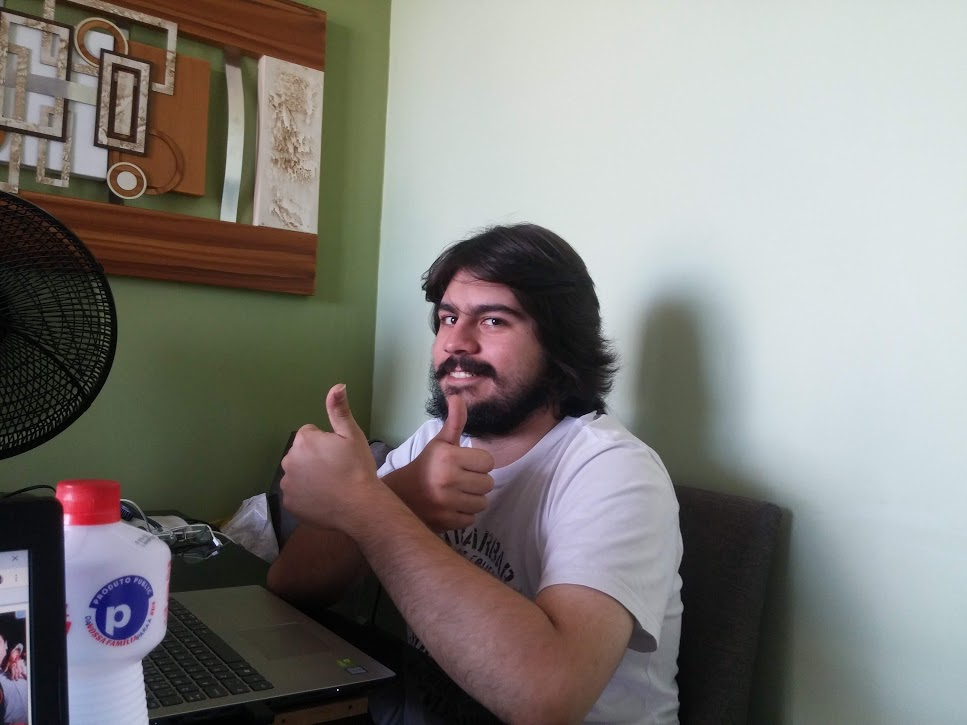
\includegraphics[height=0.85\textheight]{image/Heck.png}
    	\end{figure}
    \end{frame}

    \begin{frame}{Figuras}
        \begin{columns}
            \begin{column}{0.5\linewidth}
                \justify
                \begin{itemize}[<+->]
                    \item O pacote \emph{graphicx} deve ser carregado para adição de imagens
                    \item Ele permite mudanças em escala, cortes e outras ferramentas
                \end{itemize}
                \visible<+->{\lstinputlisting{../code/figure_example.tex}}
                \begin{itemize}[<+(1)->]
                    \item Para um detalhamento completo, leia a \href{https://ctan.org/pkg/graphicx?lang=en}{\usebeamercolor[fg]{title}documentação}
                \end{itemize}
            \end{column}
            \begin{column}{0.5\linewidth}
                \visible<4->{
            	\begin{figure}[!h]
        		    \centering
        			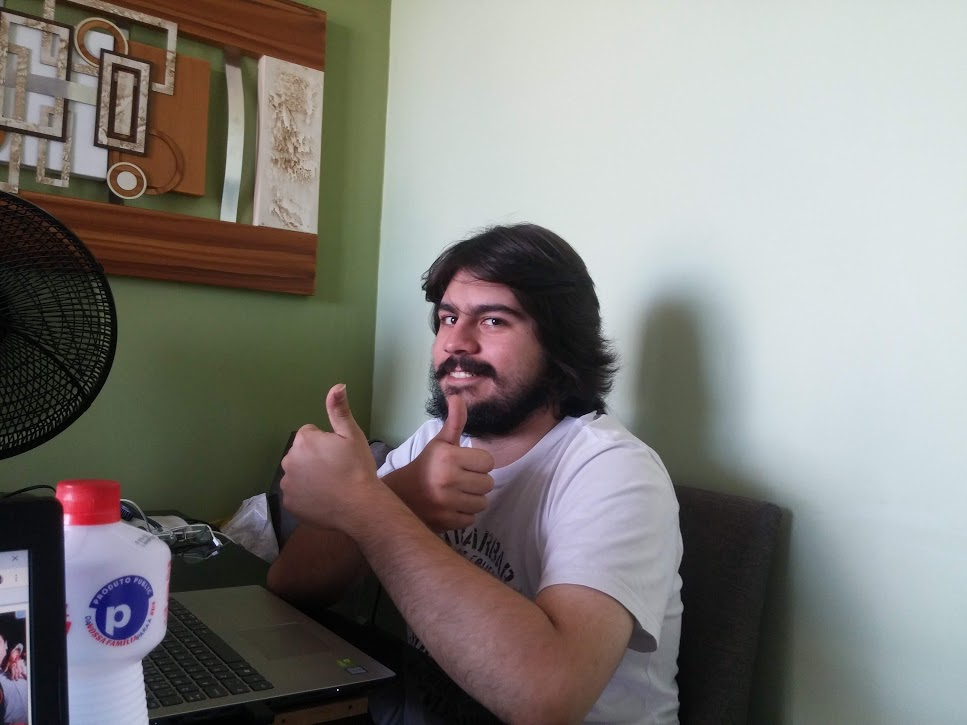
\includegraphics[height=0.75\textheight,trim={9cm 0 10cm 6cm},clip]{image/Heck.png}
        			\caption{O Professor}
            	\end{figure}}
            \end{column}
        \end{columns}
    \end{frame}

    \begin{frame}{Figuras}
        \begin{columns}
            \begin{column}{0.5\linewidth}
                \lstinputlisting{../code/figure.tex}
            \end{column}
            \pause
            \begin{column}{0.5\linewidth}
                \fbox{\begin{minipage}[c][0.8\textheight][t]{0.9\textwidth}
                    \centering
                    \vspace{0.05\textwidth}
                    \begin{columns}
                        \begin{column}{0.8\textwidth}
                            \justify
                            \fontsize{3.75}{4.5}\selectfont
                            	\begin{figure}[!h]
                        		    \centering
                        			\includegraphics[
                        			    width=0.45\linewidth,
                        			    trim={9cm 0 10cm 6cm},
                        			    clip
                        			    ]%
                        			    {image/Heck.png}\\
                        			\vspace{1.5em}
                        			Figura 1: O Professor
                            	\end{figure}
                        \end{column}
                    \end{columns}
            		\vfill
                    \fontsize{3.75}{4.5}\selectfont
                    1
                    \vspace{0.1\textwidth}
        		\end{minipage}}
            \end{column}
        \end{columns}
    \end{frame}


    \setbeamercolor{structure}{fg=slideYellow}
    \subsection{Equações}
    \begin{frame}{Equações \visible<2->{bagunçadas}}
        \begin{equation*}
            \imath\hbar\cdot\frac{\partial}{\partial t}\Psi\left(\vec{r},t\right) = \left[\frac{-\hbar^2}{2\mu}\cdot\nabla^2 + V\left(\vec{r},t\right)\right]\cdot\Psi\left(\vec{r},t\right)
        \end{equation*}
        \begin{equation*}
            e^{\imath\pi}+1=0
        \end{equation*}
        \begin{equation*}
            F(n)=\frac{\left(\frac{1+\sqrt{5}}{2}\right)^n-\left(-\frac{2}{1+\sqrt{5}}\right)^n}{\sqrt{5}}
        \end{equation*}
        \begin{equation*}
            0.\Dot{9}=1
        \end{equation*}
        \begin{equation*}
            \sigma_F = \sqrt{\left(\frac{\partial_F}{\partial_x}\right)^2(\sigma_x^2) + \left(\frac{\partial_F}{\partial_y}\right)^2(\sigma_y^2) + \left(\frac{\partial_F}{\partial_z}\right)^2(\sigma_z^2)}
        \end{equation*}
        \begin{equation*}
            \overset{\infty}{\underset{-\infty}{\int}} \frac{1}{\sigma\sqrt{2\pi}}e^{-\frac{1}{2}\left(\frac{x-mu}{\sigma}\right)} \delta x = 1
        \end{equation*}
    \end{frame}

    \begin{frame}{Equações}
        \begin{eqnarray}
            \nonumber \imath\hbar\cdot\frac{\partial}{\partial t}\Psi\left(\vec{r},t\right) & = & \left[\frac{-\hbar^2}{2\mu}\cdot\nabla^2 + V\left(\vec{r},t\right)\right]\cdot\Psi\left(\vec{r},t\right)\\
            \nonumber e^{\imath\pi}+1 & = & 0\\
            \nonumber F(n) & = & \frac{\left(\frac{1+\sqrt{5}}{2}\right)^n-\left(-\frac{2}{1+\sqrt{5}}\right)^n}{\sqrt{5}}\\
            \nonumber 0.\Dot{9} & = & 1\\
            \nonumber \sigma_F & = & \sqrt{\left(\frac{\partial_F}{\partial_x}\right)^2(\sigma_x^2) + \left(\frac{\partial_F}{\partial_y}\right)^2(\sigma_y^2) + \left(\frac{\partial_F}{\partial_z}\right)^2(\sigma_z^2)}\\
            \nonumber \overset{\infty}{\underset{-\infty}{\int}} \frac{1}{\sigma\sqrt{2\pi}} \cdot e^{-\frac{1}{2} \cdot \left(\frac{x-\mu}{\sigma}\right)} \delta x & = & 1
        \end{eqnarray}
    \end{frame}

    \begin{frame}{Equações}
        \begin{columns}
            \begin{column}{0.5\linewidth}
                \lstinputlisting{../code/equations.tex}
                \visible<3->{\centering\href{https://en.wikibooks.org/wiki/LaTeX/Mathematics}{
                \usebeamercolor[fg]{title}{$ \mu \alpha \theta \eta \mu \alpha \tau \iota \kappa \acute\alpha $}}}
            \end{column}
            \pause
            \begin{column}{0.5\linewidth}
                \fbox{\begin{minipage}[c][0.8\textheight][t]{0.9\textwidth}
                    \centering
                    \vspace{0.05\textwidth}
                    \begin{columns}
                        \begin{column}{0.8\textwidth}
                            \justify
                            \fontsize{3.75}{4.5}\selectfont
                            \hfill$e^{i\pi} = 0$\hfill(1)\\
                        \end{column}
                    \end{columns}
            		\vfill
                    \fontsize{3.75}{4.5}\selectfont
                    1
                    \vspace{0.1\textwidth}
        		\end{minipage}}
            \end{column}
        \end{columns}
    \end{frame}

    \begin{frame}{Equações}
        \begin{equation*}
            \imath\hbar\cdot\frac{\partial}{\partial t}\Psi\left(\vec{r},t\right) = \left[\frac{-\hbar^2}{2\mu}\cdot\nabla^2 + V\left(\vec{r},t\right)\right]\cdot\Psi\left(\vec{r},t\right)
        \end{equation*}
        \pause
        \lstinputlisting{../code/schrodinger.tex}
    \end{frame}


    \setbeamercolor{structure}{fg=slideOrange}
    \subsection{Tabelas}
    \begin{frame}{Tabelas}
        \setcellgapes{2\baselineskip}
        \settowidth{\rotheadsize}{\bfseries x/x \quad}
        \begin{table}[H]
            \centering
            \resizebox{!}{0.425\textheight}{%
                \begin{tabular}{c||cccccccccccc}
                    Atividade                      & \rothead{\makecell[c]{$24/9$}} & \rothead{\makecell[c]{$1/10$}} & \rothead{\makecell[c]{$8/10$}} & \rothead{\makecell[c]{$15/10$}} & \rothead{\makecell[c]{$22/10$}} & \rothead{\makecell[c]{$29/10$}} & \rothead{\makecell[c]{$5/11$}} & \rothead{\makecell[c]{$12/11$}} & \rothead{\makecell[c]{$19/11$}} & \rothead{\makecell[c]{$26/11$}} & \rothead{\makecell[c]{$3/12$}} & \rothead{\makecell[c]{$10/12$}} \\ \hline \hline
                    \makecell{Construção\\de Hardware}         & \x &    & \x & \x & \x &    & \x &    &    &    &    &     \\ \cline{1-1}
                    \makecell{Construção\\de Software}         &    &    & \x & \x & \x &    & \x & \x &    &    &    &     \\ \cline{1-1}
                    \makecell{{ }\\{ }}Testes\makecell{\\}     & \x &    & \x & \x & \x &    & \x & \x &    & \x & \x &     \\ \cline{1-1}
                    \makecell{Ajustes dos\\Sensores}           &    &    &    & \x & \x &    & \x & \x &    & \x &    &     \\ \cline{1-1}
                    \makecell{Relatório de\\Atividades}        &    &    & \x & \x & \x &    & \x & \x &    & \x & \x &     \\ \cline{1-1}
                    \makecell{Construção do\\Relatório Final}  &    &    &    &    & \x & \x & \x & \x & \x & \x &    &     \\ \cline{1-1}
                    \makecell{Entrega do\\Relatório Final}     &    &    &    &    &    &    &    &    &    &    &    & \x  \\ \cline{1-1}
                    \makecell{{ }\\{ }}Competição\makecell{\\} &    &    &    &    &    &    &    &    &    &    &    & \x  \\ \hline
                \end{tabular}%
            }
        \end{table}
    \end{frame}

    \begin{frame}{Tabelas}
        \begin{columns}
            \begin{column}{0.5\linewidth}
                \lstinputlisting{../code/simpleTable.tex}
                \visible<3->{\usebeamercolor[fg]{title}{%
                    \begin{table}[h]
                        \centering
                        \begin{tabular}{||cc||}
                            \hline\hline
                            \href{https://www.tablesgenerator.com/}{2} & \href{https://www.tablesgenerator.com/}{1} \\
                            \href{https://www.tablesgenerator.com/}{3} & \href{https://www.tablesgenerator.com/}{4} \\ \hline\hline
                        \end{tabular}
                    \end{table}%
                }}
            \end{column}
            \pause
            \begin{column}{0.5\linewidth}
                \begin{table}[!h]
                    \centering
                    \begin{tabular}{c|c|c}
                        1 & 2 & 3 \\ \hline
                        4 & 5 & 6 \\ \hline
                        7 & 8 & 9 \\ \hline
                        * & 0 & \# \\
                    \end{tabular}
                \end{table}
            \end{column}
        \end{columns}
    \end{frame}


\section[Estruturação]{Estruturação do documento}
    \setbeamercolor{structure}{fg=slideRed}
    \subsection{Classes de Documentos}
    \begin{frame}{Classes de Documento}
        \begin{columns}
            \begin{column}{0.5\linewidth}
                Existem vários tipos de \usebeamercolor[fg]{title}{\href{https://en.wikibooks.org/wiki/LaTeX/Document_Structure}{classes de documentos}}:
                \begin{itemize}[<+->]
                    \item article
                    \item report
                    \item book
                    \item letter
                    \item beamer
                \end{itemize}
            \end{column}
            \begin{column}{0.5\linewidth}
                \visible<+->{
                Cada classe tem sua peculiaridade, como, por exemplo, \emph{article} não apresenta capítulo, apenas seções.

                Beamer tem dezenas de estilos.
                }
            \end{column}
        \end{columns}
    \end{frame}


    \subsection{Níveis do documento}
    \begin{frame}{Níveis do documento}
        \begin{columns}
            \begin{column}{0.5\linewidth}
                \lstinputlisting{../code/sectionCounters.tex}
            \end{column}
            \pause
            \begin{column}{0.5\linewidth}
                \fbox{\begin{minipage}[c][0.8\textheight][t]{0.9\textwidth}
                    \centering
                    \vspace{0.05\textwidth}
                    \begin{columns}
                        \begin{column}{0.8\textwidth}
                            \justify
                            \fontsize{4.5}{4.75}\selectfont
                            \textbf{1\hspace{1em}Seção um}\\
                            \vspace{1em}
                            \fontsize{4}{4.25}\selectfont
                            \textbf{1.1\hspace{1em}Subseção um}\\
                            \vspace{1em}
                            \fontsize{3.5}{3.75}\selectfont
                            \textbf{1.1.1\hspace{1em}Subsubseção um}\\
                            \vspace{1em}
                            \fontsize{3.5}{3.75}\selectfont
                            \textbf{Parágrafo um}\\
                            \vspace{1.5em}
                            \fontsize{3.5}{3.75}\selectfont
                            \textbf{\hspace{2em}Subparágrafo um}\\
                        \end{column}
                    \end{columns}
            		\vfill
                    \fontsize{3.75}{4.5}\selectfont
                    1
                    \vspace{0.1\textwidth}
        		\end{minipage}}
            \end{column}
        \end{columns}
    \end{frame}

    \subsection{Sumário}
    \begin{frame}{Fazendo o Sumário}
        \begin{multicols}{2}
        	\tableofcontents
        \end{multicols}
    \end{frame}

    \begin{frame}{Fazendo o sumário}
        \begin{columns}
            \begin{column}{0.5\linewidth}
                \lstinputlisting{../code/tableOfContents.tex}
            \end{column}
            \pause
            \begin{column}{0.5\linewidth}
                \fbox{\begin{minipage}[c][0.8\textheight][t]{0.9\textwidth}
                    \centering
                    \vspace{0.05\textwidth}
                    \begin{columns}
                        \begin{column}{0.8\textwidth}
                            %\justify
                            \fontsize{4.5}{5}\selectfont
                            \textbf{Contents\\}
                            \vspace{1em}
                            \fontsize{3.75}{4.5}\selectfont
                            \textbf{1\hspace{1em}Seção um\hfill 1\\}
                            \fontsize{3.75}{4.5}\selectfont
                            \hspace{1.5em}1.1\hspace{1em}Subseção um\hspace{1.75em}.\quad.\quad.\quad.\quad.\quad.\quad.\quad.\quad.\quad.\quad.\quad.\quad.\quad.\quad.\quad.\quad.\quad.\quad.\hfill 1\\
                            \fontsize{3.75}{4.5}\selectfont
                            \hspace{4em}1.1.1\hspace{1em}Subsubseção um\quad.\quad.\quad.\quad.\quad.\quad.\quad.\quad.\quad.\quad.\quad.\quad.\quad.\quad.\quad.\quad.\hfill 1

                            \vspace{2em}
                            \fontsize{4.5}{4.75}\selectfont
                            \textbf{1\hspace{1em}Seção um}\\
                            \vspace{1em}
                            \fontsize{4}{4.25}\selectfont
                            \textbf{1.1\hspace{1em}Subseção um}\\
                            \vspace{1em}
                            \fontsize{3.5}{3.75}\selectfont
                            \textbf{1.1.1\hspace{1em}Subsubseção um}\\
                            \vspace{1em}
                            \fontsize{3.5}{3.75}\selectfont
                            \textbf{Parágrafo um}\\
                            \vspace{1.5em}
                            \fontsize{3.5}{3.75}\selectfont
                            \textbf{\hspace{2em}Subparágrafo um}\\
                        \end{column}
                    \end{columns}
            		\vfill
                    \fontsize{3.75}{4.5}\selectfont
                    1
                    \vspace{0.1\textwidth}
        		\end{minipage}}
            \end{column}
        \end{columns}
    \end{frame}


    \setbeamercolor{structure}{fg=slidePink}
    \subsection{Referências cruzadas}
    \begin{frame}{Referências cruzadas}
        \begin{columns}
            \begin{column}{0.5\linewidth}
                \lstinputlisting{../code/crossref.tex}
            \end{column}
            \pause
            \begin{column}{0.5\linewidth}
                \fbox{\begin{minipage}[c][0.8\textheight][t]{0.9\textwidth}
                    \centering
                    \vspace{0.05\textwidth}
                    \begin{columns}
                        \begin{column}{0.8\textwidth}
                            \justify
                            \fontsize{4.5}{4.75}\selectfont
                            \textbf{1\hspace{1em}Seção um}\\
                            \vspace{1em}
                            \fontsize{3.5}{3.75}\selectfont
                            Bom dia, bebê. Não esqueça o dejejum!\\ \vspace{1em}
                            \fontsize{4.5}{4.75}\selectfont
                            \textbf{2\hspace{1em}Seção dois}\\
                            \vspace{1em}
                            \fontsize{3.5}{3.75}\selectfont
                            Mas não se apresse. Lembra do que eu disse em 1?\\
                        \end{column}
                    \end{columns}
            		\vfill
                    \fontsize{3.75}{4.5}\selectfont
                    1
                    \vspace{0.1\textwidth}
        		\end{minipage}}
            \end{column}
        \end{columns}
    \end{frame}

    \begin{frame}{Referências cruzadas}
        \begin{itemize}[<+->]
            \item Imagens e tabelas são consideradas objetos flutuantes
            \item Para selecionar a localização preferencial, utilizar as chaves [ ]
            \begin{description}[<+->]
                \item[h] \emph{here}: no local onde foi invocado no texto
                \item[t] \emph{top}: no topo de página de invocação
                \item[b] \emph{bottom}: na base da página de invocação
                \item[p] \emph{page}: centralizado em página própria
            \end{description}
            \item O processamento de localização é feita pelo compilador, então você \textit{deve} referenciar as imagens pelo índice no texto.
            \item Normalmente imagens são colocadas nos apêndices
            \item Então, escrever coisas como ``na imagem abaixo'' é \only<beamer|-.>{idiota}\visible<+->{incoerente}
        \end{itemize}
    \end{frame}

    \subsection{Referências bibliográficas}
    \begin{frame}{Referências bibliográficas}
        \begin{columns}
            \begin{column}{0.5\linewidth}
                \lstinputlisting{../code/biblatex.tex}
            \end{column}
            \pause
            \begin{column}{0.5\linewidth}
                \fbox{\begin{minipage}[c][0.8\textheight][t]{0.9\textwidth}
                    \centering
                    \vspace{0.05\textwidth}
                    \begin{columns}
                        \begin{column}{0.8\textwidth}
                            \justify
                            \fontsize{3.5}{3.75}\selectfont
                            O sólido de Einstein da referência (1) é muito louco.\\
                            \vspace{2em}
                            \fontsize{4.5}{4.75}\selectfont
                            \textbf{Referências}\vspace{-2.5em}
                            \begin{table}[h!]
                                \centering
                                \begin{tabular}{rp{0.8\textwidth}}
                                    1& EINSTEIN, A. Die Plancksche Theorie der Strahlung und\\
                                     & die Theorie der spezifischen Wa\"{r}rm.\textbf{Annalen de Physik},\\
                                     & v.~327,n.~1, p.~180-190, 1907.~Disponível em:\\
                                     & \texttt{https://onlinelibrary.wiley.com/doi/abs/10.1002/}\\
                                     & \texttt{andp.19063270110}. Acesso em:~20~dez.~2018.
                                \end{tabular}
                            \end{table}
                        \end{column}
                    \end{columns}
            		\vfill
                    \fontsize{3.75}{4.5}\selectfont
                    1
                    \vspace{0.1\textwidth}
        		\end{minipage}}
            \end{column}
        \end{columns}
    \end{frame}


    \begin{frame}{O arquivo de bibliografia}
        \begin{columns}
            \begin{column}{0.5\linewidth}
                \lstinputlisting{../code/referencias.bib}
            \end{column}
            \pause
            \begin{column}{0.5\linewidth}
                \justify
                \begin{itemize}[<+->]
                    \item Deve conter todas as informações que a ABNT exige! A \href{http://ftp.inf.utfsm.cl/pub/tex-archive/macros/latex/contrib/abntex2/doc/abntex2cite.pdf}{\usebeamercolor[fg]{title}{ABNTeX2}} pode ajudar
                    \item A google pode gerar as entradas tanto para \href{https://scholar.google.com}{\usebeamercolor[fg]{title}{artigos}} quanto para \href{https://books.google.com}{\usebeamercolor[fg]{title}{livros}}
                    \item Em último recurso, você pode gerar com uma \href{https://truben.no/latex/bibtex/}{\usebeamercolor[fg]{title}{ferramenta online}}.
                \end{itemize}
            \end{column}
        \end{columns}
    \end{frame}


\setbeamercolor{structure}{fg=slidePurple}
\section{Finalizando}
    \subsection{O template oficial}
    \begin{frame}{O template da equipe}
        \begin{columns}
            \begin{column}{0.5\linewidth}
                \justify
                \begin{itemize}[<+->]
                    \item O template da equipe tem alguns comando especiais, criados especialmente para lá.
                    \item Em destes é o ambiente \emph{names}, que cria uma lista de alinhada.
                    \item Criação de ambientes é algo avançado, muito legal para explorar, mas não agora
                    \item Neste momento, abrimos o template o mostramos tudo\dots
                \end{itemize}
            \end{column}
            \begin{column}{0.5\linewidth}
                \visible<2->{\lstinputlisting{../code/nomes.tex}}
            \end{column}
        \end{columns}
    \end{frame}

    \subsection{Sobre a atividade}
    \begin{frame}{Finalização}
        \begin{columns}
            \begin{column}{0.5\linewidth}
                \justify
                Seu currículo deve conter:
                \begin{itemize}[<+->]
                    \item Foto (sim, foto)
                    \item Nome em tamanho grande (como fazer tamanho grande? Veja o livro!)
                    \item Sua equação favorita
                    \item Uma tabela com as coisas que você já fez na vida (curta!)
                    \item Imagens, equações e tabelas deves ser referenciadas do texto
                \end{itemize}
            \end{column}
            \begin{column}{0.5\linewidth}
                \justify
                \begin{itemize}[<+->]
                    \item Vocês terminaram o currículo?
                    \item Ele está \impecavel?
                    \item Preciso conferir, vamos ver se pegaram
                    \item Façam perguntas
                \end{itemize}
            \end{column}
        \end{columns}
    \end{frame}

    \begin{frame}
        \centering
        \VERYHuge{\usebeamercolor[fg]{title}Mãos à obra}
    \end{frame}

 %    \subsection*{Sobre o professor}
 %    \setbeamercolor{structure}{fg=darkgray}
	% \begin{frame}{Sobre o professor}
	% 	\begin{itemize}
	% 		\item Técnico de mecatrônica - ETEC Jorge Street - 2014
	% 		\item Ingressante de 2015
	% 		\item Programador na equipe UFABC Rocket Design
	% 		\item Ciência da Computação
	% 		\item Engenharia de Informação
	% 		\item Entusiasta de tecnologia
	% 	\end{itemize}
	% 	Agradecimento especial a \emph{Alexandre Olivieri}, sem o qual, esta apresentação não ficaria pronta a tempo.
%    \end{frame}